% Options for packages loaded elsewhere
\PassOptionsToPackage{unicode}{hyperref}
\PassOptionsToPackage{hyphens}{url}
\PassOptionsToPackage{dvipsnames,svgnames,x11names}{xcolor}
%
\documentclass[
  11pt,
  letterpaper,
]{article}
\usepackage{amsmath,amssymb}
\usepackage{iftex}
\ifPDFTeX
  \usepackage[T1]{fontenc}
  \usepackage[utf8]{inputenc}
  \usepackage{textcomp} % provide euro and other symbols
\else % if luatex or xetex
  \usepackage{unicode-math} % this also loads fontspec
  \defaultfontfeatures{Scale=MatchLowercase}
  \defaultfontfeatures[\rmfamily]{Ligatures=TeX,Scale=1}
\fi
\usepackage{lmodern}
\ifPDFTeX\else
  % xetex/luatex font selection
\fi
% Use upquote if available, for straight quotes in verbatim environments
\IfFileExists{upquote.sty}{\usepackage{upquote}}{}
\IfFileExists{microtype.sty}{% use microtype if available
  \usepackage[]{microtype}
  \UseMicrotypeSet[protrusion]{basicmath} % disable protrusion for tt fonts
}{}
\makeatletter
\@ifundefined{KOMAClassName}{% if non-KOMA class
  \IfFileExists{parskip.sty}{%
    \usepackage{parskip}
  }{% else
    \setlength{\parindent}{0pt}
    \setlength{\parskip}{6pt plus 2pt minus 1pt}}
}{% if KOMA class
  \KOMAoptions{parskip=half}}
\makeatother
\usepackage{xcolor}
\usepackage[margin=1in]{geometry}
\usepackage{longtable,booktabs,array}
\usepackage{calc} % for calculating minipage widths
% Correct order of tables after \paragraph or \subparagraph
\usepackage{etoolbox}
\makeatletter
\patchcmd\longtable{\par}{\if@noskipsec\mbox{}\fi\par}{}{}
\makeatother
% Allow footnotes in longtable head/foot
\IfFileExists{footnotehyper.sty}{\usepackage{footnotehyper}}{\usepackage{footnote}}
\makesavenoteenv{longtable}
\usepackage{graphicx}
\makeatletter
\def\maxwidth{\ifdim\Gin@nat@width>\linewidth\linewidth\else\Gin@nat@width\fi}
\def\maxheight{\ifdim\Gin@nat@height>\textheight\textheight\else\Gin@nat@height\fi}
\makeatother
% Scale images if necessary, so that they will not overflow the page
% margins by default, and it is still possible to overwrite the defaults
% using explicit options in \includegraphics[width, height, ...]{}
\setkeys{Gin}{width=\maxwidth,height=\maxheight,keepaspectratio}
% Set default figure placement to htbp
\makeatletter
\def\fps@figure{htbp}
\makeatother
\setlength{\emergencystretch}{3em} % prevent overfull lines
\providecommand{\tightlist}{%
  \setlength{\itemsep}{0pt}\setlength{\parskip}{0pt}}
\setcounter{secnumdepth}{5}
\newlength{\cslhangindent}
\setlength{\cslhangindent}{1.5em}
\newlength{\csllabelwidth}
\setlength{\csllabelwidth}{3em}
\newlength{\cslentryspacingunit} % times entry-spacing
\setlength{\cslentryspacingunit}{\parskip}
\newenvironment{CSLReferences}[2] % #1 hanging-ident, #2 entry spacing
 {% don't indent paragraphs
  \setlength{\parindent}{0pt}
  % turn on hanging indent if param 1 is 1
  \ifodd #1
  \let\oldpar\par
  \def\par{\hangindent=\cslhangindent\oldpar}
  \fi
  % set entry spacing
  \setlength{\parskip}{#2\cslentryspacingunit}
 }%
 {}
\usepackage{calc}
\newcommand{\CSLBlock}[1]{#1\hfill\break}
\newcommand{\CSLLeftMargin}[1]{\parbox[t]{\csllabelwidth}{#1}}
\newcommand{\CSLRightInline}[1]{\parbox[t]{\linewidth - \csllabelwidth}{#1}\break}
\newcommand{\CSLIndent}[1]{\hspace{\cslhangindent}#1}
\ifLuaTeX
\usepackage[bidi=basic]{babel}
\else
\usepackage[bidi=default]{babel}
\fi
\babelprovide[main,import]{spanish}
% get rid of language-specific shorthands (see #6817):
\let\LanguageShortHands\languageshorthands
\def\languageshorthands#1{}
\usepackage[utf8]{inputenc}
\usepackage{hyperref}
\hypersetup{urlcolor = blue, citecolor = blue,linkcolor=blue}
\usepackage{floatrow}
\floatsetup[figure]{capposition=top}
\usepackage{longtable}
\usepackage{array}
\usepackage{multirow}
\usepackage{dcolumn}
\usepackage{float}
\usepackage{booktabs}
\usepackage{longtable}
\usepackage{array}
\usepackage{multirow}
\usepackage{wrapfig}
\usepackage{float}
\usepackage{colortbl}
\usepackage{pdflscape}
\usepackage{tabu}
\usepackage{threeparttable}
\usepackage{threeparttablex}
\usepackage[normalem]{ulem}
\usepackage{makecell}
\usepackage{xcolor}
\ifLuaTeX
  \usepackage{selnolig}  % disable illegal ligatures
\fi
\IfFileExists{bookmark.sty}{\usepackage{bookmark}}{\usepackage{hyperref}}
\IfFileExists{xurl.sty}{\usepackage{xurl}}{} % add URL line breaks if available
\urlstyle{same}
\hypersetup{
  pdftitle={Problem Set 3: Making Money with ML?},
  pdfauthor={Gustavo Adolfo Castillo Álvarez (201812166),; Alexander Almeida Ramírez (202225165),; Jorge Luis Congacha Yunda (201920042) y; Jaime Orlando Buitrago González (200612390)},
  pdflang={es},
  colorlinks=true,
  linkcolor={Maroon},
  filecolor={Maroon},
  citecolor={Blue},
  urlcolor={Blue},
  pdfcreator={LaTeX via pandoc}}

\title{Problem Set 3: Making Money with ML?}
\usepackage{etoolbox}
\makeatletter
\providecommand{\subtitle}[1]{% add subtitle to \maketitle
  \apptocmd{\@title}{\par {\large #1 \par}}{}{}
}
\makeatother
\subtitle{Big Data y Machine Learning para Economía Aplicada}
\author{Gustavo Adolfo Castillo Álvarez (201812166), \and Alexander Almeida Ramírez (202225165), \and Jorge Luis Congacha Yunda (201920042) y \and Jaime Orlando Buitrago González (200612390)}
\date{2024-05-26}

\begin{document}
\maketitle

\hypertarget{introducciuxf3n}{%
\section{Introducción}\label{introducciuxf3n}}

En su \textit{paper}, Rosen (1974) proporciona una aproximación metodológica (econométrica) para estimar precios hedónicos. Más específicamente, explora los equilibrios del mercado y las decisiones de los agentes y los efectos en el bienestar para evidenciar la relación entre los precios de los bienes y sus diferentes características. Esta fue una contribución importante para estimar los precios (Hedónicos) de los bienes a partir de las características o atributos (precios implícitos) a partir de la observación de los precios de bienes heterogéneos sus características asociadas.

Como uno de los \textit{papers} más citados del \textit{Journal of Political Economy} (Greenstone, 2017), se obtiene una aproximación al comportamiento de la oferta y demanda (equilibro) a partir del proceso generador de datos entre los bienes y sus características. Para el mercado inmobiliario -en el que los comportamientos de los agentes, oferta y demanda, y equilibrios no se pueden explicar en su totalidad con la teoría microeconómica convencional-, esta aproximación ha sido de singular importancia, más aún en el contexto de la ciudad de Bogotá.

Así por ejemplo, Perdomo (2011) utiliza los precios hedónicos cómo método econométrico para estimar el precio de las viviendas y posteriormente el de la cercanía a Transmileno; Carriazo et~al. (2013) identifican cómo de no incluir la calidad del aire en las estimación a través de precio hedónicos conlleva un sesgo en los precios de las viviendas en Bogotá. Lozano \& Anselin (2012) utilizan variables espaciales en los submercados de la viviendas para estimar los precios en Bogotá, identificando una gran capacidad predictiva, pero afectada (sobre estimación) por los estratos socioeconómicos. También se encuentran Medina et~al. (2007) quienes demuestran como los subsidios aplicados a las tarifas de los servicios públicos se transfieren al precio de las viviendas.

Esta breve exploración bibliográfica refleja los usos y potencialidades de la contribución de Rosen (1974) al mercado inmobiliario con énfasis en la ciudad de Bogotá. Claro está, como la capital de Colombia, Bogotá es una ciudad heterogénea con dinámicas poblacionales, sociales y económicas distribuidas a por todo el territorio urbano, las cuales pueden afectar los precios del mercado inmobiliario. Más aun, en una localidad como Chapinero, la cual es una de las áreas centrales de la ciudad; con una gran catnidad de población flotante; donde se cuenta con vías que se conectan con el sistema de movilidad de la ciudad; se tienen usos del suelo asociados a actividades comerciales y residenciales; y se tienen parques, canales y corredores ecológicos (Decreto 468, 2006).

Por estas características, tal vez Chapinero sea la localidad con la mayor complejidad de formas de habitar el territorio de la ciudad del país, lo cual la hace un espacio geográfico donde convergen múltiples factores que afectan los precios de las viviendas. Por tal razón, construir uno o varios modelos predictivos de los precios es desafiante y una necesidad, ante una potencial inversión que compre la mayor cantidad de predios, gastando lo menos posible.

Ahora bien, para construir el o los modelos se utilizó una muestra de los anuncios publicados en la página web \href{ https://www.properati.com.co/}{Properati}. Este sitio web de origen argentino y con presencia en varios países de Latinoamérica, le permite a propietarios publicar un bien inmueble con la mayor cantidad de información (precio, características y amenidades, ubicación y descripción), y a personas interesadas en adquirir o arrendar un bien contactarse con el comprador. Es decir, se utilizó una página web que ofrece servicios de intermediación, pero que permite caracterizar la oferta de bienes en Bogotá.

De igual manera, se utilizó la información de Open Street Map (transporte público, comercio, equipamentos colectivos, y vías y trasnporte público), la cual permitió asociar información geográfica relevante a la muestra de \href{ https://www.properati.com.co/}{Properati}. Así como se utilizó también la información de la página web Infraestructura de Datos Espaciales de Bogotá (Ideca), un portal de libre acceso y consulta de la Unidad Administrativa Especial de Catastro Distrital (UAECD), de donde se utilizaron las bases de datos (capas) de las localidades de Bogotá

Con estas fuentes de información se construyeron diferentes modelos para predecir el precio de las viviendas en Chapinero. Estos modelos aplican los conceptos abordados en la clase \textit{Big Data y Machine Learning para Economía Aplicada}, los cuales se describen con mayor detalle en las siguientes secciones. En las siguientes secciones adicionalmente se encuentran: la presentación de las bases de datos utilizadas, presentando a su vez estadísticas descriptivas que facilitan su comprensión; los resultados obtenidos luego de su impelmentación; y unas conclusiones de todo el ejercicio.

Resultados\ldots{}

\hypertarget{datos-y-muxe9todos}{%
\section{Datos y Métodos}\label{datos-y-muxe9todos}}

Los datos principales consistieron en los archivos descargados de la página de datos de la \href{https://www.kaggle.com/competitions/uniandes-bdml-202410-ps3}{Competencia en Kaggle}. Esta base de datos contiene 48.930 observaciones, distribuidas en 10.286 observaciones para prueba (21\%) y 38.644 para entrenamiento (79\%). Cada observación representa un inmueble para venta publicado en \href{ https://www.properati.com.co/}{Properati} entre 2019 y 2021 en la ciudad de Bogotá. Dentro de las características de cada inmueble se tienen las áreas (construida y cubierta), el número de habitaciones y baños, el tipo de propiedad (casa o apartamento), y el título y descripciónn con el que se hizo la publicación en la página web y localización (latitud y longitud). Dada la estructura de la base de datos es muy probable que se haya construido a través de un ejercicio de \textit{Web Scrapping} y luego se haya dispuesto para su descarga y uso en el Problem Set 3.

A partir de las descripciones, se utilizó el análisis de texto para constrastar el tipo de inmueble publicado con el que se encuentra en la descripción, extraer el número de pisos de las casas, e identificar el piso en el que se encuentran los apartamentos. Como se tienen todos los inmuebles para Bogotá, en función de su localización (latitud y longitud), se extrajeron aquellas casas y apartamentos dentro de la localidad de Chapinero. Este ejercio se realizó mediante la extracción los de puntos (capa construida con la latitud y longitud) dentro del polígono de Cahpinero (capa del Ideca). Al cruzar la capa de los polígonos las localidades con la tabla de \emph{test} observamos que 593 propiedades se encuentran fuera de Chapinero (Figura \ref{fig:train-chapi-dots}), que es la localidad en la cuál se predecirán los precios de las viviendas.

\begin{figure}[H]
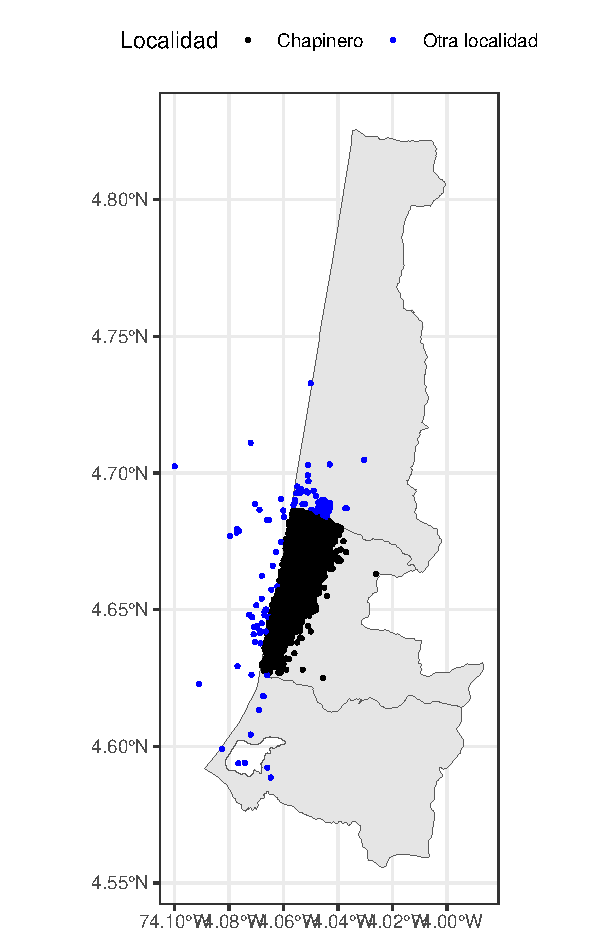
\includegraphics[width=0.7\linewidth]{../views/figures/train_dots} \caption{Ubicación datos de validación}\label{fig:train-chapi-dots}
\end{figure}

Utilizando el mismo método de análisis espacial, se utilizaron las capas de Open Street Maps para medir las distancias del inmueble a gimnasios, estaciones de Transmilenio, bares, supermercados, colegios, hospitales, principales avenidas, centros comerciales y universidades.Las principales estasdísticas descriptivas según los tipos de bienes inmuebles se ven a continuación:

\begin{table}[!h]
\centering
\caption{\label{tab:descriptive-tbl}Estadísticas descriptivas}
\centering
\begin{tabular}[t]{l|c|c|c|c}
\hline
Variable & Promedio & Desv. est. & Mín & Máx.\\
\hline
Precio (millones) & 847.2 & 375.8 & 300.0 & 1650.0\\
\hline
Área cubierta (\$km\textasciicircum{}2\$) & 128.4 & 45.4 & 31.0 & 505.0\\
\hline
Área total (\$km\textasciicircum{}2\$) & 137.4 & 1088.0 & 15.0 & 108800.0\\
\hline
Habitaciones & 2.5 & 0.8 & 1.0 & 11.0\\
\hline
Baños & 2.7 & 0.9 & 1.0 & 7.0\\
\hline
Dromitorios & 2.4 & 1.0 & 0.0 & 11.0\\
\hline
Número de pisos & 1.0 & 0.1 & 1.0 & 6.0\\
\hline
Piso & 2.1 & 3.0 & 1.0 & 60.0\\
\hline
Dist. parque (\$km\$) & 159.9 & 95.5 & 4.7 & 1948.5\\
\hline
Dist. Transmilenio (\$km\$) & 801.1 & 476.3 & 0.3 & 2968.8\\
\hline
Dist. bar (\$km\$) & 1149.1 & 470.1 & 1.5 & 2297.6\\
\hline
Dist. colegio (\$km\$) & 481.3 & 300.7 & 0.0 & 2271.6\\
\hline
Dist. avenida (\$km\$) & 230.2 & 228.4 & 0.0 & 2074.1\\
\hline
Dist. universidad (\$km\$) & 725.4 & 411.7 & 0.0 & 2768.8\\
\hline
Dist. gimnasio (\$km\$) & 730.1 & 402.4 & 10.2 & 2685.6\\
\hline
Dist. CAI(\$km\$) & 560.3 & 312.6 & 3.8 & 1680.2\\
\hline
Dist. supermercados (\$km\$) & 531.5 & 289.6 & 0.0 & 2142.9\\
\hline
Dist. hospitales (\$km\$) & 830.2 & 415.6 & 0.0 & 3408.1\\
\hline
Dist. centro comercial (\$km\$) & 247.0 & 188.6 & 1.1 & 2428.6\\
\hline
\end{tabular}
\end{table}

Para la localidad de Chapinero, luego del procedimiento anterior, se obtuvo una base de datos con 10.000 observaciones. En total, se obtuvieron 9.702 (97\%) apartmentos y 298 (3\%) casas en venta. En promedio, los inmuebles fueron publicados a un precio de 847,1 millones, tienen 137,4\(mt^2\) de área construida, 128,3\(mt^2\) de área habitables, 2,4 habitaciones, 2,6 baños y 2,3 dormitorios. Las amenidades más cercanas son los parques a una distancia promedio de 159,9 metros, centros comerciales a de 246,9 metros y las avenidas a 230,2 metros. Las más lejanas son los bares a 1,1 km, seguido por los hospitales (830 m) y las estaciones de transmileno (801 m).

Sobre este último hallazgo, esta oferta de bienes inmuebles puede estar caracterizada por casas o apartamentos más alejadas de las zonas con mayor flujo de población flotante. Al ser una localidad en la que en su centralidad alberga la mayor oferta de universidades de Bogotá, así como donde se desarrollan actividades comerciales, los inmuebles destinados a usos residenciales que se ofrecen en el mercado se encuentran más alejados de esta centralidad. Claro está, se tiene una heterogénea composición, pues como se observa en la tabla anterior aproximadante las desviaciones estándar de las distancias son la mitad de los valores promedio, y se obtienen distancia en un rango de entre 0 m 3 km.

\hypertarget{modelo-y-resultados}{%
\section{Modelo y resultados}\label{modelo-y-resultados}}

En esta sección se exponen los modelos que se utilizaron para predecir los precios de la vivienda en la localidad de Chapinero, las variables utilizadas en los modelos y la selección de hiperparámetros. En particular, se utilizaron los modelos de bosques, bosques aleatorios, regresión lineal, elasticnet y boosting para realizar la predicción. Finalmente, se presenta una comparación del rendimiento de estos modelos. El mejor resultado se obtuvo con el modelo de Random Forest utilizando como métrica el Mean Absolute Error metric (MAE).

\hypertarget{modelo-y-descripciuxf3n-de-las-variables}{%
\subsection{Modelo y descripción de las variables}\label{modelo-y-descripciuxf3n-de-las-variables}}

Para todos los modelos utilizados para la predicción, se utilizó el siguiente modelo:

\[
Precio= f(\text{características propias}, \text{características del vecindario},\text{variables temporales})
\]
\textless\textless\textless\textless\textless\textless\textless{} Updated upstream

Siguiendo a Mendieta López \& Perdomo (2007), se utilizaron tres categorías de variables que capturan atributos que explican el precio de la vivienda. El primero, corresponde a variables que capturan características convencionales d elas viviendas como el número de habitaciones, el número de baños, la superficie total y el tipo de propiedad. El segundo grupo está conformado por características del vecindario que corresponde a criterios de seguridad, por ejemplo, la distancia de la vivienda al Comando de Atención Inmediata(CAI), a criterios de servicios, como la distancia a parques, centros comeciales, instituciones educativas, y de accesibilidad de transporte, por ejemplo, distancia a la estación del transmilenio. Las variables de distancia fueron calculadas utilizando la paqueteria Osmadata del programa R. A continuación, se presenta una tabla con la descripción de las variables:

Siguiendo a Mendieta López \& Perdomo (2007), se utilizaron tres categorías de variables que capturan atributos que explican el precio de la vivienda. El primero, corresponde a variables que capturan características convencionales d elas viviendas como el número de habitaciones, el número de baños, la superficie total y el tipo de propiedad. El segundo grupo está conformado por características del vecindario que corresponde a criterios de seguridad, por ejemplo, la distancia de la vivienda al Comando de Atención Inmediata(CAI), a criterios de servicios, como la distancia a parques, centros comeciales, instituciones educativas, y de accesibilidad de transporte, por ejemplo, distancia a la estación del transmilenio. Las variables de distancia fueron calculadas utilizando la paqueteria Osmadata del programa R. El tercero, corresponde a factores de geolocalización,como la longitud y la latitud) y temporales, como el mes y el año, debido a que los precios pueden variar por el ciclo económico. A continuación, se presenta una tabla con la descripción de las variables:

\begin{table}[ht]
\centering
\caption{Nombres de las variables y su descripción}
\begin{tabular}{|c|c|}
\hline
Nombre de la variable & Descripción  \\
\hline
\hline
bathrooms\_median & Número de baños de la vivienda \\
\hline
surface\_total\_median & Área total de la vivienda  \\
\hline
property\_type & =1 si la vivienda corresponde a una casa \\
distancia\_avenida_\principal & Dato 5 \\
\hline
distancia\_parque & Distancia de la vivienda al parque más cercano \\
\hline
distancia\_comercial & Distancia de la vivienda al cento comercial más cercano \\
\hline
distancia\_avenida\_principal & Distancia de la vivienda a la avenida principal\\
\hline
distancia\_universidad & Distancia de la vivienda a la universidad más cercana \\
\hline
distancia\_cai & Distancia de la vivienda al CAI de policía más cercano \\
\hline
distancia\_bar & Distancia de la vivienda al bar más cercano \\
\hline
distancia\_gimnasio & Distancia de la vivienda al gimnasio más cercano \\
\hline
distancia\_transmi & Distancia de la vivienda a la estación de transmilenio más cercana \\
\hline
distancia\_SM & Distancia de la vivienda al Supermercado más cercano \\
\hline
distancia\_colegio & Distancia de la vivienda al colegio más cercano \\
\hline
distancia\_hospitales & Distancia de la vivienda al hospital más cercano \\
\hline
month,year & Año-mes  \\
\hline
lat,lon & Coordenadas de geolocalización de la casa \\
\hline
\end{tabular}
\end{table}

\hypertarget{descripciuxf3n-del-modelo}{%
\subsection{Descripción del modelo}\label{descripciuxf3n-del-modelo}}

\hypertarget{comparativa-con-otros-modelos}{%
\subsection{Comparativa con otros modelos}\label{comparativa-con-otros-modelos}}

Además del modelo finalmente escogido, se ejecutaron otras técnicas para realizar la predicción de los precios de la vivienda en Chapinero. Se utilizaron para todos los otros modelos las mismas variables explicativas descritas en la tabla anexo. Se estimaron las siguientes técnicas adicionales al random forest: regresión lineal, Elastic net, Boosting y árboles de decisión. Para todos estos modelos, se utiliza un cross-validation con 10 particiones con el fin de

\begin{table}[ht]
\centering
\caption{Comparativa con otros modelos}
\begin{tabular}{lcccccr}
\hline \hline
Estadística & Random Forest & RL & Linear Regression & Elastic Net & Boosting & Decision tree \\
\hline
MAE (Kaggle) & 223834975 & 308749889 & 260870545 & 289260591 & 304528484 & 279848874 \\
RMSE & 185392301 & 258160495 & 210281690 & 266505969 & 282794569 & 240176517 \\
MAE(train) & 125757655 & 191380688 & 143548002 & 200055282 & 216060881 & 178784207 \\
\hline
\end{tabular}
\end{table}

\hypertarget{conclusiones}{%
\section{Conclusiones}\label{conclusiones}}

El presente estudio realizó un

\hypertarget{referencias-bibliogruxe1ficas}{%
\section{Referencias bibliográficas}\label{referencias-bibliogruxe1ficas}}

\hypertarget{refs}{}
\begin{CSLReferences}{1}{0}
\leavevmode\vadjust pre{\hypertarget{ref-dec468}{}}%
Alcaldía Mayor de Bogotá. (20 de noviembre de 2006). \emph{Por el cual se reglamenta la UPZ 99, Chapinero, ubicada en la loclaidad Chapinero} (Decreto 468 de 2006, Ed.).

\leavevmode\vadjust pre{\hypertarget{ref-carriazo}{}}%
Carriazo, F., Ready, R., \& Shortle, J. (2013). Using stochastic frontier models to mitigate omitted variable bias in hedonic pricing models: A case study for air quality in Bogotá, Colombia. \emph{Ecological Economics}, \emph{91}, 80-88.

\leavevmode\vadjust pre{\hypertarget{ref-greenstone}{}}%
Greenstone, M. (2017). The Continuing Impact of Sherwin Rosen's {«Hedonic Prices and Implicit Markets: Product Differentiation in Pure Competition»}. \emph{Journal of Political Economy}, \emph{125}(6), pp. 1891-1902.

\leavevmode\vadjust pre{\hypertarget{ref-lozano}{}}%
Lozano, n., \& Anselin, L. (2012). Is the price right?: Assessing estimates of cadastral values for Bogotá, Colombia. \emph{Regional Science. Policy \& Practice}, \emph{4}(4), 495-508.

\leavevmode\vadjust pre{\hypertarget{ref-medina}{}}%
Medina, C., Morales, L., Bernal, r., \& Torero, M. (2007). Stratification and Public Utility Services in Colombia: Subsidies to Households or Distortion of Housing Prices? {[}with Comments{]}. \emph{Economía}, \emph{7}(2), 41-99.

\leavevmode\vadjust pre{\hypertarget{ref-mendieta}{}}%
Mendieta López, J. C., \& Perdomo, J. A. (2007). \emph{Especificaci{ó}n y estimaci{ó}n de un modelo de precios hed{ó}nico espacial para evaluar el impacto de Transmilenio sobre el valor de la propiedad en Bogot{á}}.

\leavevmode\vadjust pre{\hypertarget{ref-perdomo}{}}%
Perdomo, J. (2011). A methodological proposal to estimate changes of residential property value: case study developed in Bogotá. \emph{Applied Economics Letters}, \emph{18}(16), 1577-1581.

\leavevmode\vadjust pre{\hypertarget{ref-rosen}{}}%
Rosen, S. (1974). Hedonic Prices and Implicit Markets: Product Differentiation in Pure Competition. \emph{Journal of Political Economy}, \emph{82}(1), 34-55.

\end{CSLReferences}

\hypertarget{repositorio}{%
\section{Repositorio}\label{repositorio}}

El respositorio se puede consultar en el siguiente enlace:

\begin{itemize}
  \item \href{https://github.com/guscastilloa/PS3_Repo-G3}{Problem Set 3: Making Money with ML?}
\end{itemize}

\end{document}
